
\documentclass[3p]{elsarticle}

\usepackage{amsmath}
\usepackage{amssymb}
\usepackage{amsthm}
\usepackage{tikz}
\usepackage{pgfplots}

\pgfplotsset{compat=1.18}

\newtheorem{proposition}{Proposition}

\makeatletter
\def\ps@pprintTitle{%
  \let\@oddhead\@empty
  \let\@evenhead\@empty
  \let\@oddfoot\@empty
  \let\@evenfoot\@empty
}
\makeatother

\begin{document}

\title{Fiscal Dominance and Asset Price Redistribution}

\author{H\'ector J. Villarreal}
\address{Tec de Monterrey}

\begin{abstract}
This paper studies the distributional consequences of fiscal dominance through asset prices.
When public debt constrains monetary policy, interest rates may decline as debt increases.
Lower discount rates raise asset valuations, generating capital gains for asset holders.
In a simple framework combining public debt dynamics, fiscal reaction functions, and a
debt-sensitive interest rate rule, we derive a formal condition under which fiscal dominance
generates redistribution toward asset-owning households through the asset price channel,
and show that the wealth share of asset holders is increasing in public debt.
\end{abstract}

\maketitle

\section{Introduction}

Public debt has reached historically high levels in many advanced and emerging economies.
At the same time, the global environment of ultra-low interest rates that prevailed during
much of the past two decades appears to be fading. As borrowing costs increase, concerns
about debt sustainability and the interaction between fiscal and monetary policy have
re-emerged. In particular, recent policy discussions have revived interest in the possibility
of \emph{fiscal dominance}, a regime in which monetary policy becomes constrained by the
need to maintain government debt sustainability.

Under fiscal dominance, interest rate policy may respond not only to macroeconomic
stabilization objectives but also to the fiscal position of the government. When public
debt is high, increases in interest rates raise debt servicing costs and can threaten
fiscal sustainability. In such circumstances, monetary authorities may face pressure to
keep interest rates lower than would otherwise be implied by conventional policy rules.
While this mechanism may help stabilize public finances in the short run, it may also
generate important distributional effects.

This paper highlights a simple but largely overlooked channel through which fiscal
dominance can affect the distribution of wealth. If higher public debt leads to lower
equilibrium interest rates, discount rates decline and asset prices increase. Because
ownership of financial assets is typically concentrated among a subset of households,
this asset price channel can generate redistribution toward asset holders. In this
sense, fiscal adjustment through interest rate suppression may operate not through
inflation or taxation, but through changes in asset valuations.

The analysis contributes to three strands of literature. First, it relates to the literature
on fiscal dominance and monetary--fiscal interactions (Sargent and Wallace, 1981; Leeper,
1991; Bianchi and Melosi, 2019). Second, it connects to the macroeconomic debate on public
debt sustainability in low interest rate environments (Blanchard, 2019; Dabla-Norris et al.,
2023; Eggertsson, Mehrotra, and Robbins, 2019). Third, it relates to the asset-pricing
literature emphasizing the role of discount-rate movements in asset valuation (Campbell and
Shiller, 1988; Cochrane, 2011). Greenwald, Leombroni, Lustig, and Van Nieuwerburgh (2024)
show empirically that declining interest rates generate capital gains on long-duration assets
that increase financial wealth inequality---a channel closely related to the mechanism
formalized here. Recent work on public sector balance sheets also highlights
the importance of low government funding costs in high-debt environments (Chien, Cole, and
Lustig, 2024). The practical relevance of these concerns is underscored by the OECD Global
Debt Report (OECD, 2025), which documents record sovereign bond issuance and rising
interest-payment-to-GDP ratios across member countries, conditions under which fiscal
dominance becomes an increasingly plausible policy regime.

To illustrate the mechanism, we develop a simple framework combining public debt dynamics,
a fiscal reaction function, and a debt-sensitive interest rate rule reflecting fiscal
dominance. The model shows that when interest rates decline as government debt increases,
asset prices rise mechanically through the discounting channel. If only a fraction of
households owns these assets, the resulting valuation gains increase wealth concentration.

The remainder of the paper is organized as follows. Section~2 presents the theoretical
framework. Section~3 derives the main results. Section~4 discusses the distributional
implications and policy interpretation.

\section{Model}

Consider a simple economy in discrete time. Government debt evolves according to

\begin{equation}
D_{t+1} = (1+r_t-g)D_t - PB_t
\end{equation}

where $D_t$ denotes public debt, $r_t$ the real interest rate, $g$ the growth rate of the
economy, and $PB_t$ the primary balance.

Fiscal policy responds imperfectly to public debt according to

\begin{equation}
PB_t = \alpha + \psi D_t
\end{equation}

where $\psi \geq 0$ measures the responsiveness of the primary balance to debt. A low
value of $\psi$ reflects limited fiscal adjustment capacity.

Under fiscal dominance, monetary policy becomes sensitive to the fiscal position of the
government. We capture this mechanism through a debt-sensitive interest rate rule

\begin{equation}
r_t = r^{*} - \phi D_t
\end{equation}

where $r^{*}$ denotes the benchmark interest rate and $\phi>0$ measures the strength
of monetary accommodation induced by debt pressure. This reduced-form rule captures the
implicit response of a monetary authority facing a debt-sustainability constraint. When
public debt is high, raising the policy rate increases debt-service costs and threatens
fiscal solvency, creating pressure to accommodate below the benchmark rate. Bianchi and
Melosi (2019) provide theoretical foundations for this mechanism, showing that lack of
monetary--fiscal coordination generates systematically lower rates in high-debt regimes.
Empirically, the rule is consistent with the Bank of Japan's yield curve control after
2013 and the ECB's implicit spread management during 2012--2022.

A simple extension introduces a debt threshold $\bar{D}$ such that fiscal pressures
affect interest rates only when debt exceeds a prudential level,

\[
r_t = r^{*} - \phi \max(D_t - \bar{D},\; 0),
\]

capturing the idea that fiscal dominance becomes relevant only once debt surpasses a
critical level. This formulation maps naturally onto the empirical literature on nonlinear
fiscal reaction functions and debt limits.

There exists a financial asset paying a constant dividend $A>0$. The asset price follows
a perpetuity discounting relation

\begin{equation}
P_t = \frac{A}{r_t}
\end{equation}

This is the simplest possible discounting structure. A richer Gordon growth specification,
$P_t = A/(r_t - g_A)$, would not alter the directional result of Proposition~1---only the
magnitude of $\partial P_t / \partial D_t$---and would connect naturally to the $r-g$
debt-sustainability framework of Blanchard (2019).

Substituting equation (3) into (4) yields

\begin{equation}
P_t = \frac{A}{r^{*}-\phi D_t}
\end{equation}

Finally, suppose only a fraction $\lambda \in (0,1)$ of households owns the asset.
Aggregate wealth of asset holders is

\begin{equation}
W_t = \lambda P_t
\end{equation}

\section{Results}

The relationship between public debt and asset prices follows directly from equation (5).

\begin{proposition}
Suppose $A>0$, $\phi>0$, and $r^{*}-\phi D_t>0$. Then asset prices satisfy

\[
\frac{\partial P_t}{\partial D_t} = \frac{A\phi}{(r^{*}-\phi D_t)^2} > 0.
\]

Thus, under fiscal dominance, an increase in public debt raises asset prices through the
discount-rate channel.
\end{proposition}

\textbf{Proof.}

From equation (5),

\[
P_t = A(r^{*}-\phi D_t)^{-1}.
\]

Differentiating with respect to $D_t$ gives

\[
\frac{\partial P_t}{\partial D_t}
=
\frac{A\phi}{(r^{*}-\phi D_t)^2}.
\]

Since $A>0$, $\phi>0$, and $r^{*}-\phi D_t>0$, the derivative is strictly positive.
\hfill $\square$

\medskip

Figure~\ref{fig:mechanism} illustrates the mechanism. The left panel shows the convex
relationship between public debt and asset prices. The right panel shows that the marginal
effect $\partial P_t / \partial D_t$ is itself increasing in $D_t$: the impact of fiscal
dominance on asset valuations accelerates as debt rises.

\begin{figure}[ht]
\centering
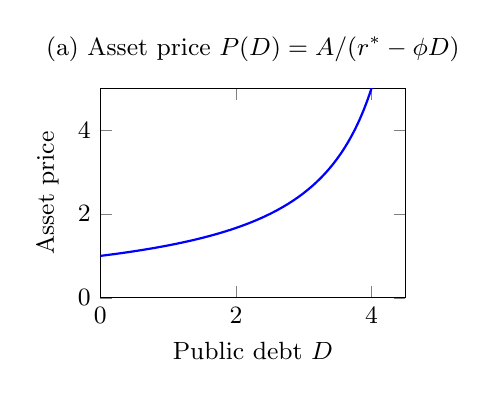
\begin{tikzpicture}
\begin{axis}[
  width=0.45\textwidth,
  height=0.35\textwidth,
  xlabel={Public debt $D$},
  ylabel={Asset price},
  xmin=0, xmax=4.5,
  ymin=0, ymax=5,
  domain=0:4.4,
  samples=200,
  title={(a) Asset price $P(D)=A/(r^{*}-\phi D)$},
  title style={font=\small},
  label style={font=\small},
  tick label style={font=\small},
]
\addplot[thick, blue] {1/(1-0.2*x)};
\end{axis}
\end{tikzpicture}
\hfill
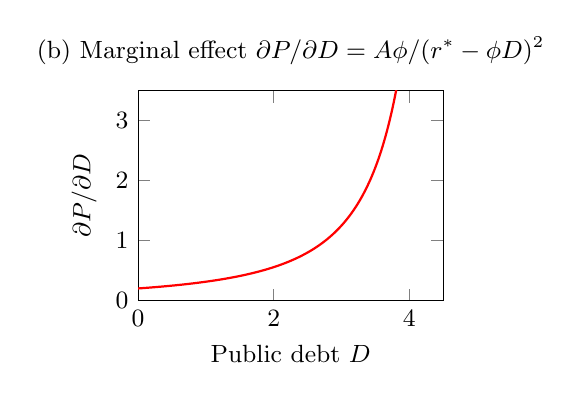
\begin{tikzpicture}
\begin{axis}[
  width=0.45\textwidth,
  height=0.35\textwidth,
  xlabel={Public debt $D$},
  ylabel={$\partial P/\partial D$},
  xmin=0, xmax=4.5,
  ymin=0, ymax=3.5,
  domain=0:4.4,
  samples=200,
  title={(b) Marginal effect $\partial P/\partial D = A\phi/(r^{*}-\phi D)^2$},
  title style={font=\small},
  label style={font=\small},
  tick label style={font=\small},
]
\addplot[thick, red] {0.2/(1-0.2*x)^2};
\end{axis}
\end{tikzpicture}
\caption{Asset price and its marginal debt sensitivity under fiscal dominance.
Parameters: $A=1$, $r^{*}=1$, $\phi=0.2$.}
\label{fig:mechanism}
\end{figure}

The distributional consequence follows formally from Proposition~1.

\begin{proposition}
Under the conditions of Proposition~1, the wealth of asset-holding households satisfies

\[
\frac{\partial W_t}{\partial D_t}
=
\frac{\lambda A\phi}{(r^{*}-\phi D_t)^2} > 0.
\]

Furthermore, let $\bar{W}$ denote the wealth of non-asset-holding households, assumed
invariant to the discount-rate channel. Define the wealth share of asset holders as
$\sigma_t = W_t/(W_t + \bar{W})$. Then $\partial \sigma_t / \partial D_t > 0$: fiscal
dominance increases the wealth share of asset-holding households.
\end{proposition}

\textbf{Proof.}

From equation (6) and Proposition~1,

\[
\frac{\partial W_t}{\partial D_t}
= \lambda \frac{\partial P_t}{\partial D_t}
= \frac{\lambda A\phi}{(r^{*}-\phi D_t)^2} > 0.
\]

For the wealth share: since $\bar{W}>0$ is independent of $D_t$,

\[
\frac{\partial \sigma_t}{\partial D_t}
=
\frac{\bar{W}}{(W_t+\bar{W})^2}
\cdot
\frac{\partial W_t}{\partial D_t}
> 0.
\]

\hfill $\square$

\section{Distributional Implications and Policy Interpretation}

The model highlights a simple redistribution channel operating through asset prices in
high-debt environments. When fiscal pressures induce monetary accommodation, lower
interest rates increase asset valuations through the discount-rate channel. Because
ownership of financial assets is typically concentrated among a subset of households,
these valuation gains accrue disproportionately to asset holders, as established in
Proposition~2.

This mechanism complements existing discussions of high public debt, which often emphasize
inflation, taxation, or fiscal consolidation as adjustment margins. The analysis suggests
that changes in asset prices may also play an important role in shaping the distributional
consequences of high-debt regimes. In this sense, fiscal adjustment through interest rate
suppression operates not through explicit redistribution, but through changes in asset
valuations that benefit households with existing financial wealth.

An important determinant of the strength of fiscal dominance is demographic structure.
In aging economies, rising old-age dependency ratios increase pension and health
expenditures, driving debt accumulation and raising the effective value of $\phi$.
Simultaneously, demographic shifts may depress the natural rate of interest $r^{*}$
through changes in aggregate saving behavior (Eggertsson, Mehrotra, and Robbins, 2019).
These forces are particularly relevant for middle-income economies undergoing rapid
fertility decline, where fiscal adjustment capacity is limited and the demographic
transition may compress the timeline over which fiscal dominance becomes binding.

The assumption that non-asset-holder wealth $\bar{W}$ is invariant to the discount-rate
channel is a simplification. If public transfers to non-asset-holding households are
themselves constrained by the debt dynamics that generate fiscal dominance, the
redistributive effect identified in Proposition~2 is amplified. Quantification of these
interactions, and of the redistribution magnitude more broadly, requires micro data on
asset ownership and a calibrated overlapping-generations framework---a natural direction
for subsequent research, particularly for emerging economies where such data remain scarce.

\section*{References}

Bianchi, F., Melosi, L., 2019. The dire effects of the lack of monetary and fiscal
coordination. Journal of Monetary Economics 104, 1--22.

Blanchard, O., 2019. Public debt and low interest rates.
American Economic Review 109, 1197--1229.

Campbell, J., Shiller, R., 1988. The dividend-price ratio and expectations of
future dividends and discount factors.
Review of Financial Studies 1, 195--228.

Chien, Y., Cole, H., Lustig, H., 2024. The return on government debt and public
sector balance sheets. NBER Working Paper.

Cochrane, J., 2011. Presidential address: Discount rates.
Journal of Finance 66, 1047--1108.

Dabla-Norris, E., et al., 2023. High public debt: Challenges and policy options.
International Monetary Fund.

Eggertsson, G., Mehrotra, N., Robbins, J., 2019. A model of secular stagnation:
Theory and quantitative evaluation.
American Economic Journal: Macroeconomics 11, 1--48.

Greenwald, D., Leombroni, M., Lustig, H., Van Nieuwerburgh, S., 2024. Financial
and total wealth inequality with declining interest rates. NBER Working Paper 28613.

Leeper, E., 1991. Equilibria under active and passive monetary and fiscal policies.
Journal of Monetary Economics 27, 129--147.

OECD, 2025. Global Debt Report 2025. OECD Publishing, Paris.

Sargent, T., Wallace, N., 1981. Some unpleasant monetarist arithmetic.
Federal Reserve Bank of Minneapolis Quarterly Review 5, 1--17.

\end{document}
